\section{Dwi Yulianingsih(1174009)}
\subsection{Pengertian}
Sistem informasi geografis merupakan sebuah aplikasi /system pengolah data spasial yang memanfaatkan system komputerisasi dengan menggabungkan data grafis dan data atribut objek memanfaatkan peta dasar digital dengan referensi yang digunakan yaitu bumi. SIG pada dasarnya akan memunculkan dan memberi data-data yang diinginkan oleh user dimana dulunya manual yang diperbaharui menjadi data digital terkomputerisasi. System informasi geografis digunakan untuk mengumpulkan, mengubah, mengevaluasi, serta mengawasi seluruh data bumi yang dibutuhkan oleh user, dulunya data disimpan secara manual yang memungkinkan data bisa hilang/ rusak maka diperbaharui agar lebih mudah dan aman.

\subsection{Sejarah}
Sejarah dari SIG kurang lebih adalah sebagai berikut :
\begin{itemize}
\item Pada tahun 1960 ilmu computer mulai berkembang pesat dan siap digunakan untuk berbagai bidang. Ahli meteorology, geologi, dan 	geofisika mulai mengikuti perkembangan zaman dan memanfaatkannya  untuk membuat peta.
\item  Pada 1963 muncul Canadian geographic information system (CGIS) di Kanada dan menjadi system informasi geografis pertama di dunia. Dua tahun kemudian Amerika mulai mengikuti jejak Kanada dengan MIDAS-nya untuk memproses data SDA yang ada disana. 
\item Pada 1967 perkembangan awal SIG diterapkan di Ottawa, Ontario oleh departemen energi pertambangan dan sumber daya (ini merupakan perkembangan dari Canadian geographic information system yang digunakan untuk inventarisasi tanah Kanada (CLI) untuk mengetahui kemampuan memetakan informasi geologi disana).  
\item CGIS memiliki aplikasi pemetaan yang berkemampuan timpang susun atau overlay, perhitungan, pemindaian, system koordinat, dan topologi yang menyimpan atribut dan lokasional dalam berkas terpisah. CGIS ini bertahan sampai tahun 1970-an dan disempurnakan agar bisa bersaing dengan aplikasi pemetaan lain yang di keluarkan oleh vendor-vendor seperti Intergraph. 
\item Perkembangan yang terus menerus terjadi memacu pemtumbuhan SIG dapat dijalankan di workstation unix dan computer pribadi dengan standar platform yang lebih sedikit dan user yang mulai mengekplor data SIG lewat internet hingga bisa menjadi seperti sekarang.
\end{itemize}

\subsection{Koordinat}
Koordinat merupakan titik-titik yang didapat dari hasil pertemuan garis latitude dan longitude atau lintang dan bujur sehingga dapat menunjukan lokasi sebuah daerah/tempat. Pada umumnya koordinat dibedakan menjadi dua yaitu koordinat geograpik dan UTM. Di koordinat geograpik ada 3 satuan yaitu :
\begin{itemize}
\item Degree, Decimal (DD,DDDD) Contoh : S 3.56734 E 104.67235
\item Degree, Minute (DD MM,MMMM) Contoh : S 3⁰ 43,5423’ E 104 33,6445’
\item Degree, Minute, Second (DD MM SS,SS) Contoh : S 3⁰ 43’ 45,22” E104 33’ 33,25”
\end{itemize}

\begin{figure}[H]
	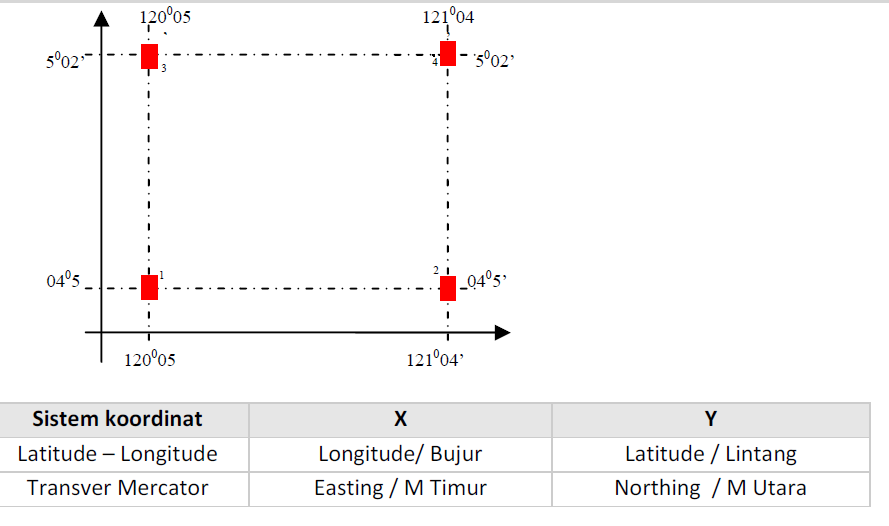
\includegraphics[width=5cm]{figures/1174009/t1.png}
	\centering
	\caption{geographic}
\end{figure}

Pada system UTM terbagi menjadi beberapa  waktu tergantung pada zonasinya, diindonesia waktu dibagi menjadi 16 zonasi seperti pada gambar di bawah :
\begin{figure}[H]
	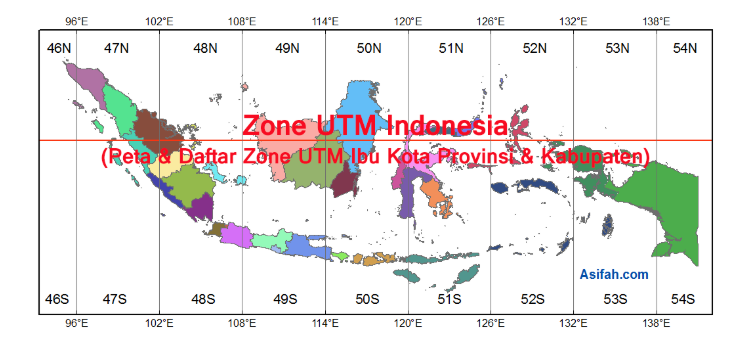
\includegraphics[width=5cm]{figures/1174009/t2.png}
	\centering
	\caption{UTM}
\end{figure}

\subsection{Data Geospasial}
Data geospasial adalah data yang memuat informasi spesifik mengenai fisik dan administrative dari sebuah objek. Aspek yang termasuk fisik disini seperti bentuk alam di permukaan (bumi) yang mengandung fenomena seperti jalan, rel kereta api, jembatan, bangunan dan sebagainya selain itu juga seperti aliran sungai, dataran tinggi, pantai, danau dan sebagainya. Termasuk juga aspek administrative seperti batas negara, pembagian wilayah, zona, postal code, batas tanah dan lainnya. Sebuah objek biasanya dikaitkan dengan atribut dari objeknya dan informasinya dapat di letakkan terpisah dengan pangkalan data induknya. Ada dua metode dalam data geospasial ini ada data vector dan data raster. Data vector terdiri dari gambaran titik geografis mau berupa titik, garis maupun polygon. Sementara data raster terdiri dari pixels yang digunakan untuk mrnggambarkan data yang berhubungan. 
\begin{figure}[H]
	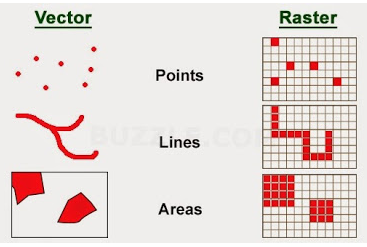
\includegraphics[width=5cm]{figures/1174009/t3.png}
	\centering
	\caption{geopasial}
\end{figure}

\subsection{Link Video}
\href{https://youtu.be/MXutHP_22_M}{Yuk lihat videonya}

\subsection{Plagiarism}
\begin{figure}[H]
	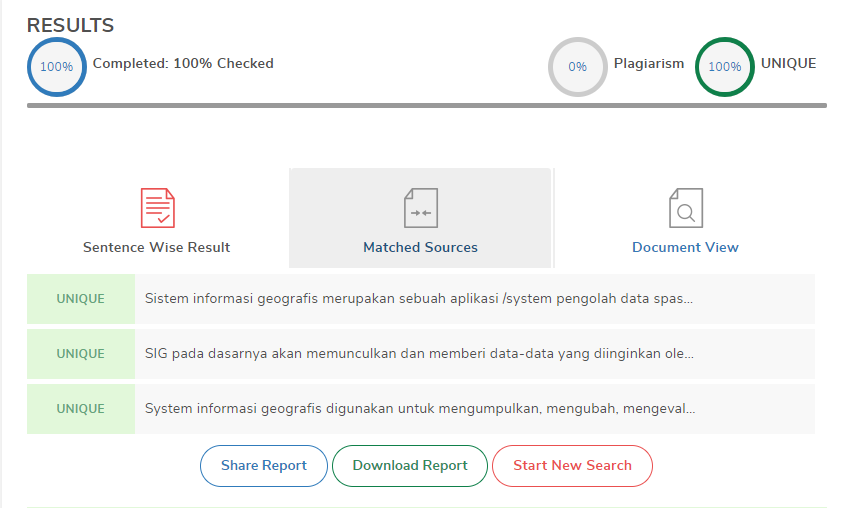
\includegraphics[width=5cm]{figures/1174009/plagiat1.png}
	\centering
	\caption{Bukti Tidak Plagiat}
\end{figure}

\begin{figure}[H]
	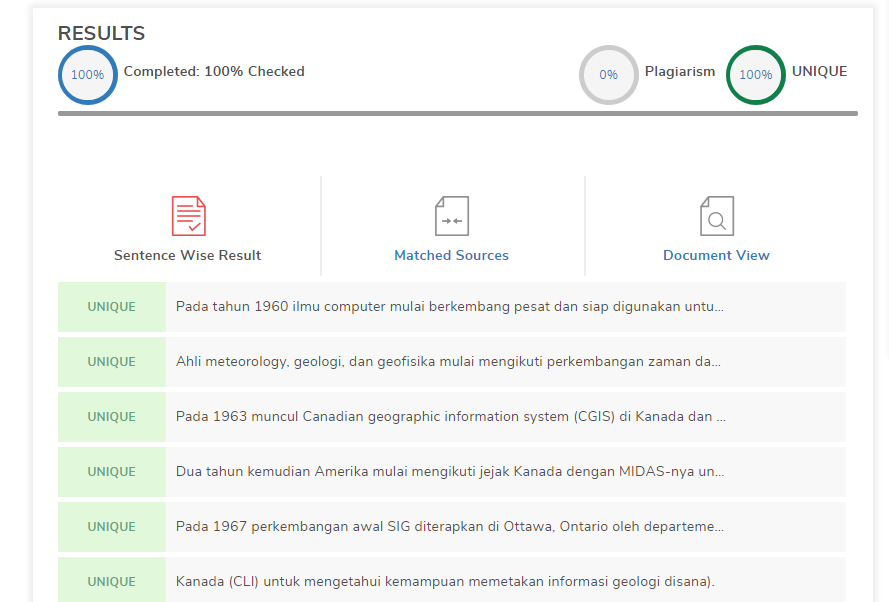
\includegraphics[width=5cm]{figures/1174009/plagiat2.png}
	\centering
	\caption{Bukti Tidak Plagiat}
\end{figure}

\begin{figure}[H]
	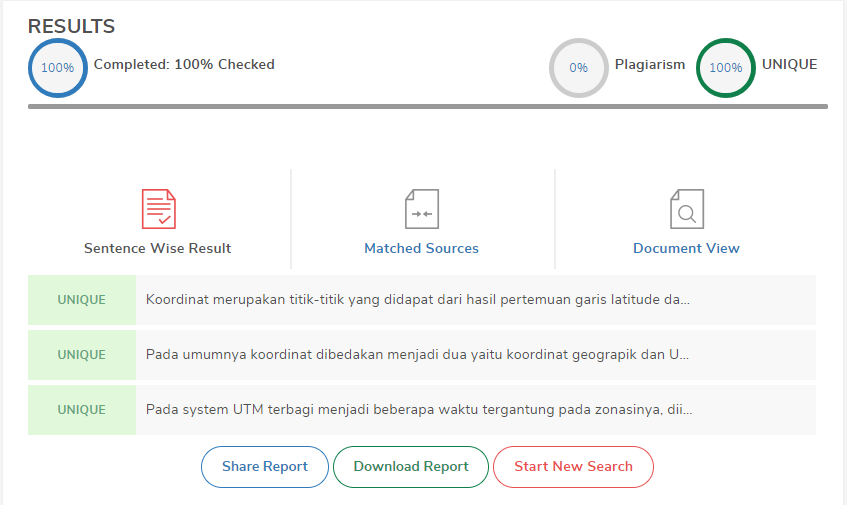
\includegraphics[width=5cm]{figures/1174009/plagiat3.png}
	\centering
	\caption{Bukti Tidak Plagiat}
\end{figure}

\begin{figure}[H]
	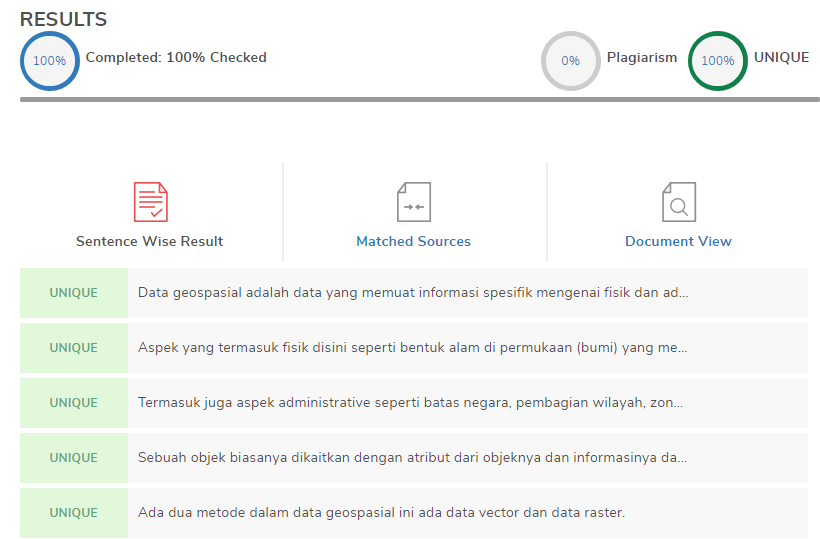
\includegraphics[width=5cm]{figures/1174009/plagiat4.png}
	\centering
	\caption{Bukti Tidak Plagiat}
\end{figure}
